%%%%%%%%%%%%%%%%%%%%%%% file template.tex %%%%%%%%%%%%%%%%%%%%%%%%%
%
% This is a template file for Web of Conferences Journal
%
% Copy it to a new file with a new name and use it as the basis
% for your article
%
%%%%%%%%%%%%%%%%%%%%%%%%%% EDP Science %%%%%%%%%%%%%%%%%%%%%%%%%%%%
%
%%%\documentclass[option]{webofc}
%%% "twocolumn" for typesetting an article in two columns format (default one column)
%
\documentclass{webofc}
\usepackage[varg]{txfonts}   % Web of Conferences font

%% Using biber in this way just breaks the class file. Frustrating!
%\usepackage[backend=bibtex]{biblatex}
% so we use ye olde natbib instead (it seems to work well enough)
\usepackage{natbib}

\begin{document}
%
\title{Modern Software Stack Building for HEP}
%
% subtitle is optionnal
%
%%%\subtitle{Do you have a subtitle?\\ If so, write it here}

\author{\firstname{Graeme A} \lastname{Stewart}\inst{1}\fnsep\thanks{\email{graeme.andrew.stewart@cern.ch}} \and
        \firstname{Benjamin} \lastname{Morgan}\inst{2}\fnsep\thanks{\email{ben.morgan@warwick.ac.uk}} \and
        \firstname{Javier} \lastname{Cervantes Villanueva}\inst{1}\fnsep \and
        \firstname{Hobbs A} \lastname{Willett}\inst{3}
        % etc.
}

\institute{CERN, 1 Esplanade des Particules, 1211 Geneva 23, Switzerland
\and
           University of Warwick, Coventry CV4 7AL, United Kindgdom 
\and
           University of Sheffield, Sheffield S10 2TN, United Kindgdom
          }

\abstract{%
High-Energy Physics has evolved a rich set of software packages that need to
work harmoniously to carry out the key software tasks needed by experiments.
The problem of consistently building and deploying these packages as a
coherent software stack is one that is shared across the HEP community. To that
end the HEP Software Foundation Packaging Working Group has worked to identify
common solutions that can be used across experiments, with an emphasis on
consistent, reproducible builds and easy deployment into CVMFS or containers
via CI systems. We based our approach on well identified use cases and
requirements from many experiments. In this paper we summarise the work of the
group in the last year and how we have explored various approaches based on
package managers from industry and the scientific computing community.

We give details about a solution based on the Spack package manager which has
been used to build the software required by the SuperNEMO and FCC experiments
and trialled for a multi-experiment software stack, Key4hep. We shall discuss
changes that needed to be made to Spack to satisfy all our requirements. We
show how support for a build environment for software developers is provided.
}
%
\maketitle
%
\section{Introduction}
\label{intro}

Software plays a critical role in the lifecycle of High-Energy Physics (HEP)
experiments. From the high-level triggers of the experiments, through the
reconstruction chain, to the identification of analysis objects, and finally to
the final physics analysis, software is ubiquitous. In parallel, the simulation
chain, generating physics events and simulating their passage through the
detector, compliments this data driven chain and is entirely done by software.

As HEP software has become more sophisticated so the dependencies on libraries
and supporting software components has become more important. This leads to the
need to build modern HEP experiment software as both a deep stack, with many
dependencies building on top of one another; and as a wide stack, with several
hundred packages in total performing many different functions.
These packages range from entirely generic
parts of a modern Linux environment, to HEP dedicated libraries, all the way up to
experiment specific code. The model of a typical HEP application is shown in
Figure \ref{fig:stack}.

\begin{figure}[h]
\centering
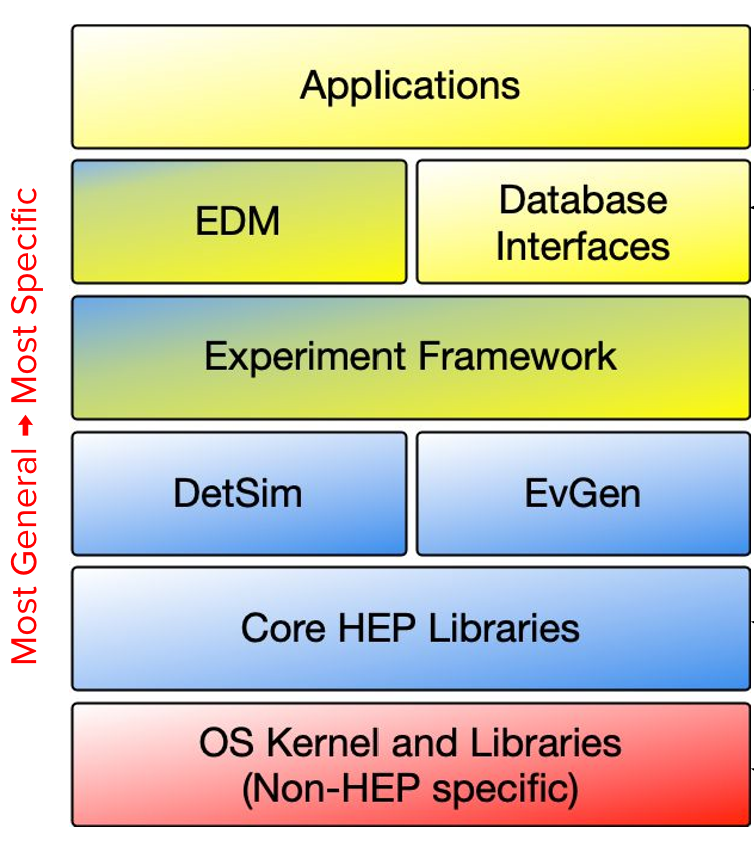
\includegraphics[width=6cm]{stack.png}
\caption{Illustrative figure showing a typical HEP software stack, with packages
categorised from most general (bottom) to most specific (top). The lowest level
components are generic to all systems, moving to scientific libraries, to common
HEP packages to, finally, experiment specific software.}
\label{fig:stack}
\end{figure}

This deep and wide set of dependencies needs to be managed carefully,
particularly for reasons of build consistency and validation (see \S\ref{hsfpwg}), thus HEP
software should be built coherently as a \emph{software stack}. As much of
this work is common between experiments, the HEP Software Foundation (HSF) has
had a long standing \emph{Packaging Working Group}\cite{HSFPWG} that has attempted to find
common solutions to this problem. In this paper we report on the recent activity
of the group and, in particular, on the Spack package manager\cite{10.1145/2807591.2807623} which is being
trialled as a possible common solution for multiple experiments.

\section{HSF Packaging Working Group}
\label{hsfpwg}

The HSF Packaging Working Group\cite{HSFPWG} was formed in 2015 to encourage communication
between the librarians of HEP experiments, who are charged with building and
maintaining their experiments' software. The group focused on:

\begin{itemize}
    \item Common build recipes and tools
    \item How to take most advantage of technologies like containers
    \item Proper support for developers and users in our collaborations
\end{itemize}

The group organised a series of meetings that reviewed packaging
practice within the experiments and also looked at different tools that
could be used for HEP stack building. These ranged from generic open 
source tools to HEP specific approaches. This early work of the group
was summarised in an HSF report \cite{l_sexton_kennedy_2016_1472340}.

In 2018 the group held a series of meetings to properly define
the use cases for packaging and deployment tools in HEP. This resulted
in the publication of the HSF Packaging Use Cases document\cite{graeme_a_stewart_2020_3634722}.
The main use cases identified were:

\begin{itemize}
    \item Build
    \begin{itemize}
        \item Builds should be completely reproducible
        \item Support for multiple build `flavours' must be available
            (e.g. for different versions of the software or for 
            using different compiler options)
        \item Toolchains and libraries should be able to be used from
            external sources (i.e. not under the control of the packaging tool)
        \item The build process should be optimised to re-use compatible
            binary artefacts from previous builds
        \item Incremental builds should be supported, where only a subset
            of packages are rebuilt (changed packages and their downstream
            dependencies)
        \item Build recipes should be easily shared between librarians
            and customised recipes should be easy to use, overriding defaults
        \item Build artefacts should be able to be stored outside of the
            build area itself and need to convey enough metadata to allow
            installation from the artefact cache without reference to the
            original build area
    \end{itemize}
    \item Deployment
    \begin{itemize}
        \item Builds must be installable to different target paths, implying
            full install time relocatability
        \item Build artefacts should be convertible to `standard' package
            formats, such as RPMs or deb packages
        \item Installations of packages built with different build options
            must be supported, without interfering with each other; however,
            it is desirable that common lower level components would only
            be installed once
        \item Removal of a release, of part of a release, must be supported
        \item It should be possible to update a release, should a fix need to
            be applied to a component
    \end{itemize}
    \item Development
    \begin{itemize}
        \item Developers should be able to compile against any deployed release
        \item Developer-built packages must take precedence in the runtime
            development environment
        \item Developers can setup an environment to recompile any external
            or component of the software stack
    \end{itemize}
\end{itemize}

These use cases can then be used when evaluating the suitability of any 
tool that can manage the build and install of a software stack for HEP.

\section{The Spack Package Manager}
\label{spack}

During 2018 and 2019 the packaging working group evaluated a number
of promising tools for building and installing HEP software. This work
built on the work of the earlier technical note from the group\cite{l_sexton_kennedy_2016_1472340}.

One tool in particular seemed to be capable of meeting most of the requirements
derived from the use cases presented above, viz.\ the Spack Package Manager,
developed by Lawrence Livermore National
Laboratory\cite{10.1145/2807591.2807623}. This tool had come to the attention
of the group shortly after the publication of HSF-TN-2016-03. Resulting
interactions between HEP package managers and librarians with the Spack
development team demonstrated a great willingness on their part to adapt to the
specific requirements of HEP and to accept patches from our community in order
to address any shortcomings that were identified.

In particular, HEP authors worked hard to improve relocation features
in Spack, to develop better support for binary caches and to chain Spack
instances together in so-called Spack chains.

Our excellent working relationship with the Spack developers resulted
in the addition of a dedicated HEP channel to the Spack Slack community.

\subsection{Key Spack Features}
\label{spack-features}

\begin{itemize}
    \item Unique hashes identifying a package's dependencies and build options
    \item Package recipes written in Python
    \item Heirarchy of build recipes supported
    \item Binary caches supported for build artefacts
    \item Use of system or externally pre-built packages
    \item Relocatable installation supported from the binary cache
    \item Use of RPATH to express dependencies in a robust way, ensuring that
        multiple versions of binares and libraries can co-exist without
        interference
    \item Downstream instances of Spack can reuse packages
        installed in an upstream Spack instance (so-called Spack chains)
\end{itemize}

Given the large feature set of Spack, the significant scientific user community
(much larger than HEP or even physics) and the postitive engagement with the
core developers, a number of HEP projects began to use the tool for their
software builds.

\section{Current Use of Spack in HEP}
\label{hep-spack-use}

\subsection{Future Circular Collider}
\label{fcc}

The Future Circular Collider\cite{Benedikt:2653673} is a next generation
accelerator project proposed for CERN that would reside in a 100km tunnel that
could house $ee$, $eh$ or $hh$ colliders. To undertake detector design studies
for experiments at FCC a full software stack is needed. At the time that the FCC
studies began the most mature software stack available was the LCG stack, built
by the CERN EP-SFT SPI project\cite{LCGStack}. Therefore, as an expedient
decision, the additional packages for FCC were built on top of exisiting
LCG releases. This required extensive use of Spack's ability to take pre-built
software, by specifiying a package's source in a "\texttt{packages.yaml}" configuration file, e.g., to
use the LCG built version of ROOT:

\begin{verbatim}
    root:
        buildable: false
        paths:{
            root@6.14.04%gcc@6.2.0
            arch=x86_64-centos7:
            /cvmfs/sft.cern.ch/lcg/releases/LCG_94/
                ROOT/6.14.04/x86_64-centos7-gcc62-opt
        }
\end{verbatim}

Once the LCG base is setup correctly, Spack then takes care of building the
additional FCC packages, as shown in Figure \ref{fig:fcc-stack}.

\begin{figure}[h]
    \centering
    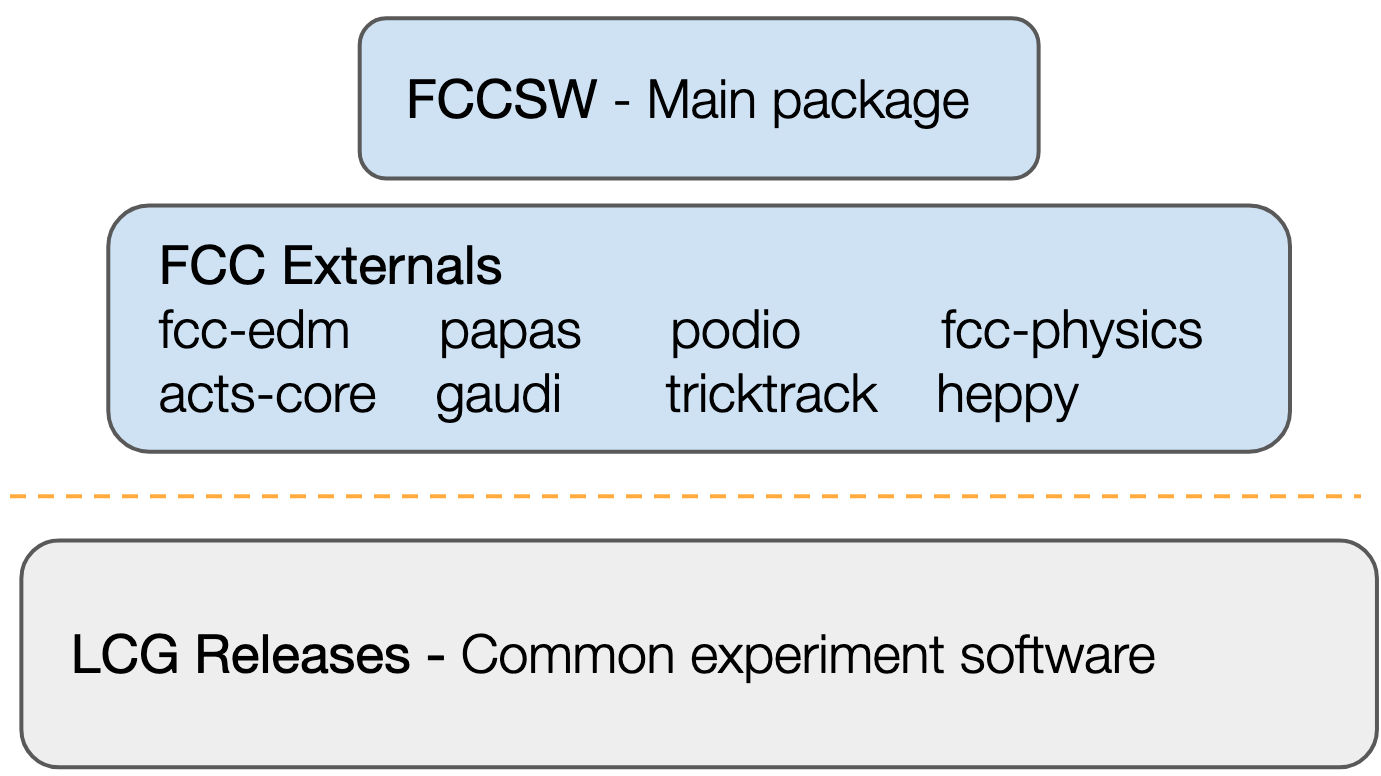
\includegraphics[width=6cm]{fcc-stack.png}
    \caption{The FCC software stack, which is built with Spack (upper blue boxes),
    but bootstraped from the CMake built LCG release (lower grey box).}
    \label{fig:fcc-stack}
\end{figure}

Once binary artefacts have been created by Spack on the build machine,
these are moved to a network filesystem that the FCC CVMFS\cite{CVMFS} master
has access to. On the CVMFS master, Spack is re-run to install and relocate
the packages into the final location under \texttt{/cvmfs/fcc.cern.ch}, where
it becomes globally accessible to users.

One problematic issue was that re-running Spack on the CVMFS master effectively
locked the architecture, e.g. \texttt{x86\_64-centos7}, to that of the CVMFS
host machine. To install for different architectures a workaround, using a
Docker container with the target architecture, was used. However, recent
enhancments to Spack have allowed an option for Spack to install for any
specified architecture, independently of the current host, so, thanks to HEP
contributors, this problem has been overcome.

Once installed in CVMFS, a simple shell script is provided that sets up the
runtime and development environment for users.

\subsection{SuperNEMO}
\label{supernemo}

SuperNEMO\cite{Piquemal2006} is a Neutrinoless Double Beta Decay experiment.
This is a small experiment, with little dedicated computing effort, so
an off-the-shelf solution for package building and distribution is very 
desirable. A previous solution, based on homebrew\cite{homebrew} had effectively
reached the limits of its capabilities.

SuperNEMO software is not currently deployed via CVMFS and the main build targets are
native OS installation and Docker containers. A wide variety of platforms are
supported: CentOS7, Ubuntu 18.04, macOS Mojave/Catalina natively; plus CentOS7
Docker/Singularity images. Similar to FCC, use is made of Spack's
\texttt{packages.yaml} feature to reuse appropriate system binaries, which greatly
reduces the build time (particularly for X11 and OpenGL packages).

Spack's hierarchical package definition features are exploited to allow for
some customised versions of particular packages, such as Qt, while relying on
the main Spack repository for the vast majority of packages.

At present, containers are built from scratch though use of a binary cache for this
and eventual CVMFS deployment is in progress.

\subsection{Key4hep Prototype}
\label{key4hep}

For studies of detectors beyond the HL-LHC era, there are different
requirements from those at running experiments. As even accelerator parameters
for ILC\cite{bambade2019international}, CLIC\cite{Boland:2210892},
FCC\cite{Benedikt:2653673} or CEPC\cite{group2018cepc} are not yet fixed, and
there are many design options available for detectors, the need is for a
software stack that is very flexible and able to rapidly be used for
physics studies of different detector options. Interest in a common solution
from multiple communities\cite{key4hep} has motivated 
building such a stack also using Spack as the prototype tool.

First of all, Spack was set to bootstrap its own build of the gcc compiler
toolchain (on the CentOS7 platform). Binary artefacts for this toolchain were
stored in a commonly accessible area for serveral independent Spack
installations. This compiler was then used to build a baseline stack of
software, that can encapsulate an HEP software workflow from event generation
though to analysis. In particular Pythia8, Geant4, DD4hep, Gaudi and ROOT were
built, with Spack itself being used to resolve and build all of the dependent
libraries and packages, which finally numbered over 100. Where necessary, build
options were specified in \texttt{packages.yaml}, so that the build was
reproducible.

After all of the binary artefacts had been built, tests were made of the 
ability to relocate all of the packages. In particular, the \texttt{RPATH}
setting for all libraries and binares was checked, to ensure that
all of the paths were valid in the relocated installation.

To setup a working runtime environment, tests were done of two solutions:

\begin{enumerate}
    \item Using a Spack \emph{view}, where a simplified installation directory
    structure (\texttt{bin}, \texttt{lib}, \texttt{include}, etc.) is created
    and softlinks to actual locations is used.
    \item Setting up a runtime \emph{module}, which uses a standard environment
    modules package (Environment Modules or lmod) to manipulate the shell environment
    to use the new software.
\end{enumerate}

Both solutions proved practical. The advantage of the view is a very compact
set of modifications to the environment. However, any additional non-standard
environment variables required need to be setup separately, so a wrapper script
needs to be provided. The advantage of the modules solution is that all special
environment settings are automatically handled by Spack and the module system.
However, the modifications to the environment are quite significant (e.g., a
very long \texttt{PATH}), which can make certain tasks unweildy.

The final production solution for runtime and development is still being
investigated, with modules favoured for development and views for production
running of jobs.

\section{Conclusions and Future Work}

The HSF Packaging Working Group has surveyed many potential solutions to the
problem of building, deploying and running large HEP software stacks. From
those studies Spack has emerged as a very promising tool. FCC was the first
experiment in HEP to demonstrate successfully how Spack can be used and even
integrated on top of other, existing solutions. CVMFS deployment was
demonstrated. SuperNEMO has shown how Spack relieves a small experiment of much
of the burden of maintianing a software build and deployment system. The
Key4hep project has provided proof-of-concept studies that a complete large
HEP software stack can be supported relatively easily, taking advantage
of Spack features and the large number of package recipes that are
maintained for and by the scientific community.

Work on utilising Spack as the package manager is now continuing, in the
context of the Key4hep project and as a replacement for the classic approach
to building the LCG stack.

\section*{Acknowledgements}

The authors would like to thank the many colleagues active in the HSF
Packaging Group, without whom this paper would not have been possible.
Special thanks are due to the original convenors of the group,
Elizabeth Sexton-Kennedy (FNAL) and Benedikt Hegner (CERN) and to
Patrick Gartung (FNAL) and Chris Green (FNAL) who have contributed
greatly to the HEP interactions with the Spack core development team.

%
% BibTeX or Biber users please use (the style is already called in the class, ensure that the "woc.bst" style is in your local directory)
\bibliography{modern-stack}

\end{document}

% end of file template.tex
